\chapter{Robó}
\label{chap:robaqua}
A integridade da infraestrutura offshore é uma questão-chave para a produção ininterrupta de petróleo e gás, bem como para a segurança dos funcionários embarcados. O envelhecimento das infraestruturas causada principalmente pela corrosão e fadiga gera um aumento da probabilidade de falha. Em casos extremos, a perda da integridade estrutural pode causar o colapso da estrutura resultando na perda completa da instalação e ocasionalmente em um desastre ecológico e humano. 

O projeto de vida típico de uma plataforma é de 20 - 25 anos, no entanto, devido à demanda atual para a produção de petróleo e gás, muitas dessas plataformas continuarão em operaçãos além do projetado. A inspeção estrutural da região submersa destas estruturas apresenta um desafio logístico dado o meio subaquático. Logo, a importância do desenvolvimento de sistemas submarinos adequados para inspeções periódicas de integridade estrutural. Um agravante a este problema é o aumento do percentual da produção executada por equipamento submersos, que resulta em uma maior demanda de inspeção periódica dos equipamentos posicionados no fundo marinho.  

Atualmente, as estruturas subaquáticas são inspecionados ou por ROVs ou mergulhadores. Ambos os métodos são dispendiosos e ineficientes, principalmente por duas razões: 
\begin{itemize}
	\item necessidade de pessoal altamente especializado;
	\item e o tempo necessário para realizar inspeções manualmente.
\end{itemize}

Portanto, o principal desafio no problema de inspeção estrutural submarina reside no desenvolvimento de um método eficiente de inspeção, que não necessita de um pessoal altamente especializado e que pode ser utilizada diretamente a partir das plataformas, sem a necessidade de uma embarcação de suporte.  


%\section{Veículos de operação remota}
%\label{chap:sotarov}
%
%\subsection{Estudo do estado da arte}
%\label{sec:sotarov}
%pybullet
%\subsubsection{Benchmarking}
%\label{ssec:benchrov}
%
%\subsubsection{Estudo de comparação das operações de ROV}
%\label{sec:comprov}
%
%\ldots

%------------------------------------------------------------

\section{Manipuladores subaquáticos}
\label{chap:sotamani}



Um manipulador, também conhecido com um braço robótico, é considerado a ferramenta mais adequada para executar operações de intervenção submarina. Assim, os veículos submarinos não tripulados (\textit{\acs{UUV}s}), como os veículos operados remotamente (ROVs) e, em alguns casos, os veículos subaquáticos autônomos (\textit{\acs{AUV}s}) são equipados com um ou mais manipuladores submarinos. UUVs com manipuladores são freqüentemente chamados de Manipulador de Veículos Subaquáticos (\textit{\acs{UVM}s}). Segundo \cite{sivvcev2018underwater}, a maioria dos manipuladores subaquáticos existentes usados ​​nos UUVs são antropomórficos, ou seja, eles são projetados para se assemelhar a um braço humano. Esses manipuladores são compostos de uma seqüência de corpos rígidos (links) interconectados por meio de juntas rotacionais com um deslocamento angular adequado entre elas e garras ou outras ferramentas intercambiáveis ​​presas no \textit{end-effector}. Para a observação de seu entorno, eles são geralmente acompanhados por um equipamento adicional composto por uma ou mais câmeras e holofotes montados no veículo subaquático da base e/ou no próprio manipulador.

Os manipuladores subaquáticos são usados ​​para uma variedade de tarefas submarinas em diferentes aplicações em petróleo e gás offshore, energia renovável e indústrias de engenharia civil marinha, bem como em ciências marinhas e aplicações militares \cite{capocci2017inspection}. Como eles estão sendo usados ​​em uma ampla gama de aplicações, os manipuladores submarinos são projetados para diferentes propósitos, por ex. existem manipuladores com mobilidade limitada equipados com garras para içar objetos grandes e pesados, manipuladores usados ​​para fixar uma garra destacável a um objeto afundado selecionado, manipuladores de garras equipados com garras ou copos de vácuo usados ​​para fixar um veículo submerso a estruturas submersas ou perto de paredes planas durante a operação, manipuladores equipados com dispositivos de inspeção, manipuladores de intervenção hábeis com garras que podem transportar diferentes ferramentas usadas para operações de reparo e manutenção em estruturas submersas etc. Geralmente, os ROVs da classe trabalhadora são equipados com dois manipuladores, na maioria dos casos simples agarrador poderoso para segurar o ROV perto da estrutura de engenharia hidráulica ou naufrágio, enquanto o outro manipulador realiza a tarefa de intervenção real.

Algumas das tarefas que os manipuladores subaquáticos são projetados para executar incluem inspeção de tubos \cite{christ2013rov}, salvamento de objetos afundados \cite{chang2004distance}, limpeza de superfícies \cite{davey1999non}, abertura e fechamento de válvulas, perfuração, corte de cabos \cite{christ2013rov}, assentamento e reparo de cabos, limpeza de entulhos e redes de pesca, biológica \cite{jones2009using} e amostragem geológica \cite{noe2006surface}, etc. Em geral, os manipuladores estão localizados na parte frontal do veículo submerso, mas nem sempre é esse o caso, por exemplo, há veículos com um manipulador localizado na parte inferior lado \cite{ribas2011girona}.

\subsection{Estudo do estado da arte}
\label{sec:sotamani}
De forma abrangente o estado da arte do conhecimento sobre os sistemas manipuladores subaquáticos foi baseado inicialmente em um artigo fundamentado por \citeonline{sivvcev2018underwater}. 

Os autores forneceram uma pesquisa sobre o uso da tecnologia de manipulação para uma variedade de operações de intervenção submarina e inspeção em diferentes áreas de aplicação offshore. Ambas as soluções de manipuladores subaquáticos comercialmente disponíveis e os sistemas de protótipos foram analisados. Tópicos relevantes foram discutidos, incluindo especificações técnicas de manipuladores, projeto mecânico, atuação, modelagem de robô (cinemática e dinâmica), abordagens de controle e algoritmos (controle de movimento, controle cinemático, planejamento de movimento) e uma comparação detalhada foi apresentada destacando vantagens e desvantagens de diferentes soluções presentes na tecnologia de manipulação submarina. Este tópico apresenta uma imagem atual da tecnologia existente a fim de fornecer uma fonte útil para futuras pesquisas no campo da robótica subaquática e manipulação. Fatores críticos que limitam o desempenho de manipuladores subaquáticos passaram a ser mais entendidos a partir da revisão abrangente deste estado da arte. Os autores recomendam fortemente que esses fatores sejam considerados durante o projeto de futuros sistemas manipuladores subaquáticos.

%fazer um mapa mental sobre os tópicos relevantes

Muitos pesquisadores \cite{wang2008novel} \cite{suboh2009modeling} \cite{golea2002fuzzy} \cite{pandian2010neuro} têm trabalhado no desenvolvimento de algoritmos de controle, mas poucos foram implementados e testados em sistemas de manipuladores submarinos físicos. 
Além disso, não há manipuladores comerciais controláveis ​​por torque no momento. Portanto, muitos dos algoritmos de controle de baixo nível propostos não são aplicáveis ​​a sistemas comerciais e até mesmo à maioria dos protótipos. Pesquisas acadêmicas relativamente recentes que incluiam ensaios submarinos experimentais em ambiente de campo ou pelo menos em tanques de teste tem sido realizada na Ocean One, MARIS, TRIDENT, RAUVI, PANDORA, CManipulator e KORDI. 
Os dois últimos tem concentrado suas pesquisas em sistemas de manipuladores de ROV hidráulicos comerciais, enquanto os restantes concentram nas intervenções de AUVs com manipuladores de protótipos elétricos. 
Alguns dos projetos em curso na atualidade estão sendo desenvolvidos em ambientes relevantes de manipulação submarina, desta forma pode-se estabelecer uma pequena lista:
%as empresas precisam ser referenciadas ou nota de rodapé
\begin{itemize}
	\item ROBUST \url{http://eu-robust.eu/};
	\item MERBOTS \url{http://www.irs.uji.es/project/merbots}; 
	\item DexROV \url{http://www.dexrov.eu/};
	\item Operations Support Engineering - MaREI \url{http://www.mmrrc.ul.ie/};
\end{itemize}
 
Destes projetos acima, a Operation Support Engineering - MaREI faz uso de manipuladores hidráulicos padrão da indústria em ROV, e o restante usa manipuladores elétricos em AUVs.

Uma visão introdutória como a apresentada acima, pode dirimir inicialmente sobre o tema de forma macro, porém para uma pesquisa mais profunda há que se levar em consideração subtópicos para que temas mais profundos possam ser estudados. Neste sentido o projeto toma como referência a divisão apresentada por \citeonline{sivvcev2018underwater} com algumas modificações em sua separação (fFigura \ref{fig:estrusub}).
 
%preparar figura dos tópicos relevantes
%------ picture -------------
%\begin{sidewaysfigure*}
\begin{figure}[H] 
  \begin{center} 
  	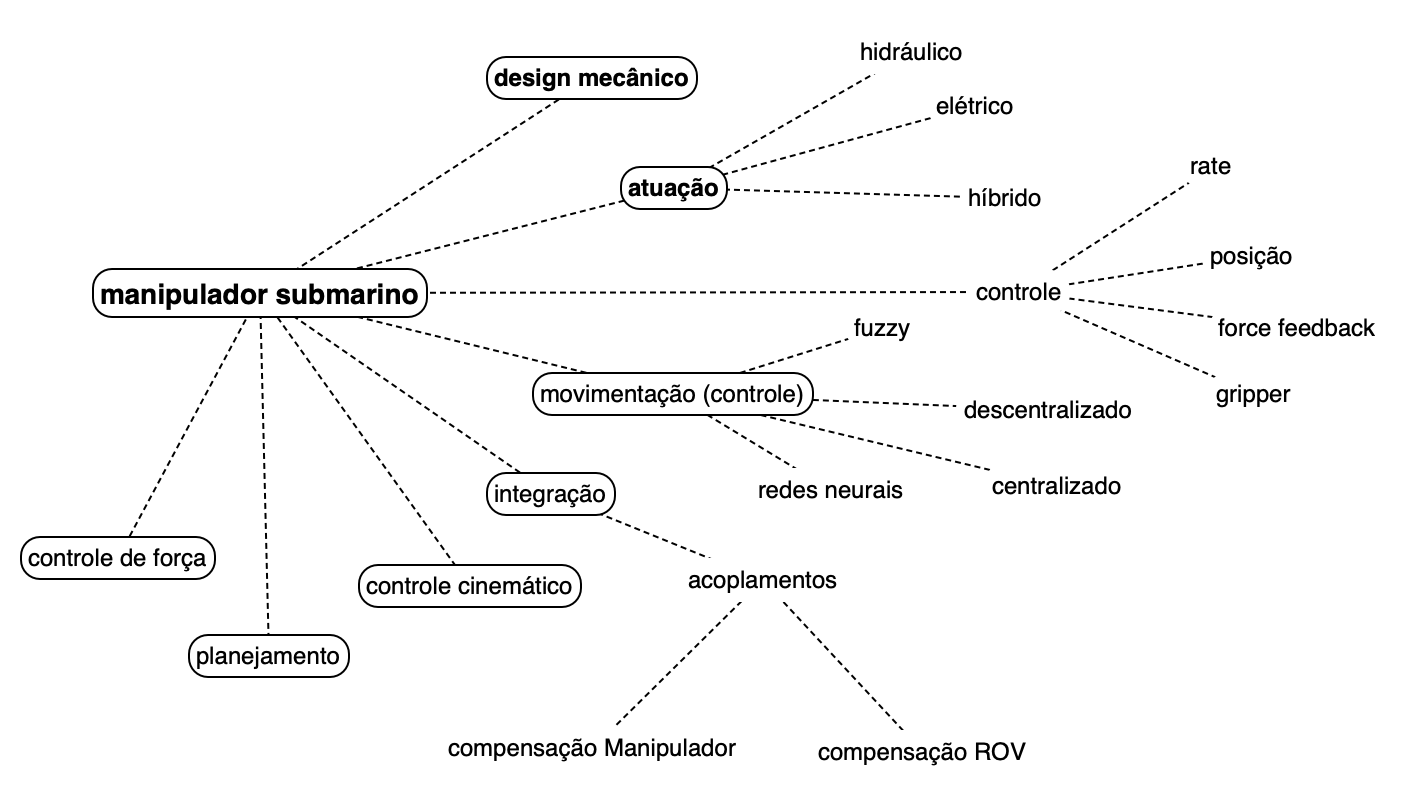
\includegraphics[width=0.9 \textwidth]{images/manipuladorsubmarino.png} 
  \end{center} 
  \caption{Estrutura de subsistemas para um manipulador submarino.} 
  %\legend{Fonte: os autores.} 
  \label{fig:estrusub} 
\end{figure}
%\end{sidewaysfigure*}
%----------------------------

\subsubsection{Design mecânico}
\label{sec:desmeca}

Os materiais mais comuns usados ​​na construção de manipuladores subaquáticos são ligas de metal, muitas vezes escolhidos por causa da alta resistência do material e propriedades contra corrosão. Com o objetivo de reduzir o peso na água e aliviar a carga dispendida pelo atuador experimentos tem sido desenvolvidos para incrementar capacidade de flutuabilidade nos manipuladores \cite{ishimi1991manipulation}.

Normalmente os manipuladores submarinos mais robustos são concebidos para atuar entre 3000 a 6500 metros da água do mar, no entanto alguns manipuladores foram desenvolvidos podendo atingir até 7000m, como é o caso do manipulador da Schilling Robotics - Titan 4 e um protótipo desenvolvido por \citeonline{zhang20147000m}.

Além disso, existem alguns sistemas projetados para a profundidade total do oceano, ou seja 11.000 metros de profundidade. O Instituto Oceanográfico Woods Hole, em colaboração com a Kraft Robotics, projetou um desses manipuladores para o propósito da missão de exploração da Mariana Trench \cite{bowen2008nereus}. Outros incluem "Magnum 7", um produto da ISE Ltd. e "The ARM" e "MK-37", desenvolvidos pela Western Space and Marine, Inc.

O tamanho dos manipuladores subaquáticos é descrito por um parâmetro chamado "Reach" que representa o comprimento de toda a cadeia cinemática do manipulador. Juntamente com a amplitude de movimento das articulações, determina o tamanho da área de trabalho do manipulador, um conjunto de pontos que podem ser alcançados pelo seu efeito final \cite{cao2011accurate}. O alcance dos manipuladores subaquáticos existentes varia de 0,5 m para os manipuladores de garras até 2,4 m para manipuladores mais robustos.

O torque máximo do punho que os manipuladores subaquáticos são capazes de produzir varia de 8Nm a 250Nm. De acordo com a ISO 13628–8:2010 \cite{iso2010petroleum}, as interfaces ROV rotativas de baixo torque em sistemas de produção submarina, que normalmente são usadas em válvulas de agulha submarinas, têm classificação máxima de 75Nm. Além disso, a capacidade de elevação de carga dos manipuladores submarinos varia de 5 kg a 500 kg. Os fabricantes costumam fornecer parâmetros diferentes para a capacidade de elevação do manipulador; o que torna a comparação não trivial, pois a capacidade de carga não é uma valor fixo, mas depende da posição do manipulador.

Em geral, o peso de um manipulador submarino não molhado está entre 6 kg e 150 kg; no entanto, seu peso na água é mais importante pois determina a flutuabilidade necessária no veículo de base para compensar o manipulador. O peso e o tamanho são fatores muito importantes, pois são diretamente responsáveis ​​pela quantidade de acoplamento dinâmico introduzido entre o manipulador e o robô submarino no qual está montado e, portanto, pode influenciar o desempenho de todo o sistema. 

Para poder explorar completamente as características do manipulador, o peso do manipulador deve ser uma porcentagem baixa o suficiente, para que o acoplamento dinâmico possa ser desprezado ou pelo menos levado em consideração como uma perturbação externa que pode ser tratado pelo posicionamento dinâmico do robô submarino (ROV). 

Maior peso e tamanho maior geram demandas mais altas com relação à robustez do sistema de propulsão de um robô submarino (ROV) quando submetido às perturbações causadas pelo acoplamento dinâmico. 

 A Tabela 2 apresenta o peso relativo do manipulador para o veículo para os ROVs comerciais pesados, médios e leves da classe comercial. Pode-se observar que essa relação é significativamente baixa, mesmo para os veículos comerciais leves da classe trabalhadora.

%tabela dos rovs com os manipuladores

Os manipuladores subaquáticos podem ser equipados com vários tipos de pinças no seu \textit{end effector}. As soluções comerciais apresentam diferentes garras intercambiáveis, cada uma com seu objetivo específico. Um tipo de garra comum é aquele com garras de ação paralela, que inclui um \textit{slot} para uma alça de barra T padrão \cite{iso2010petroleum}, e sua função principal é agarrar diferentes objetos e ferramentas em uma variedade de operações submarinas. As ferramentas geralmente são projetadas com uma barra em T exatamente para esse fim. As garras diferentes incluem garras de três ou quatro dedos, garras flutuantes de dois ou três dedos, garras de tesoura, pés de sucção, etc. Os atuadores das garras são geralmente hidráulicos e a força de garra das garras disponíveis comercialmente variam de 35 kgf a 652 kgf.

Dependendo da natureza da tarefa para a qual foram projetados, os manipuladores subaquáticos vêm com diferentes números de graus de liberdade (DOF). Os manipuladores subaquáticos comerciais e experimentais são geralmente projetados com três a seis DOFs, sem levar em consideração a mobilidade da garra. A razão para isso é que três DOFs são suficientes para alcançar uma posição arbitrária e seis DOFs para posição arbitrária e orientação do \textit{end effector} na área de trabalho \cite{spong2005robot}. 
O termo “função n” é frequentemente usado na literatura para descrever o número de atuadores contidos em um manipulador e esse termo também inclui a mobilidade da garra, portanto, por exemplo, um manipulador de sete funções significa que existem seis atuadores responsável pelo movimento do manipulador que fornece seis DOFs verdadeiros mais um atuador para a mobilidade da garra. Manipuladores subaquáticos com sete ou mais DOFs (sem mobilidade da pinça) não são muito comuns, mas existem. 

Manipuladores com 7 DOF são inerentemente redundantes do ponto de vista cinemático \cite{siciliano2010robotics}. Esse recurso pode desempenhar um papel importante na autonomia de manipuladores, pois a redundância pode ser explorada para um objetivo secundário, tal como evitar obstáculos. 

Manipuladores submarinos com 7 DOF é relatada por \citeonline{marani2009underwater} e \citeonline{ribas2015auv} e com oito DOF por \citeonline{greig1994arm}. 

Qualquer aplicação robótica de manipuladores subaquáticos requer algoritmos de planejamento e controle de modelagem cinemáticos aplicáveis. Os manipuladores subaquáticos geralmente têm estrutura mecânica de cadeia serial semelhante aos braços de manipuladores industriais. Existe muita literatura sobre a cinemática de robôs que pode ser aplicada a manipuladores subaquáticos, alguns dos quais podem ser encontrados em \citeonline{spong2005robot}; \citeonline{siciliano2010robotics}; e \citeonline{corke2011robotics}. 

Literatura adicional sobre sistemas manipuladores de veículos pode ser encontrada em \citeonline{p2014vehicle} e literatura mais específica relacionada a sistemas manipuladores de veículos subaquáticos em \citeonline{antonelli2014unrob}.

%inserir a tabele 1

\subsubsection{Atuação}
\label{sec:atua}
Na atualidade há dois caminhos importantes identificados no desenvolvimento de manipuladores submarinos, ambos apresentam vantagens e desvantagens, são eles: um baseado em óleo hidráulico e outro em atuadores elétricos. Há ainda algumas ideias apresentadas como uma combinação entre ambos, conforme apresentado por \citeonline{denket2006frontiers}.

Na grande maioria, os manipuladores baseados em óleo hidráulico são os mais tipicamente usados, mesmo assim há muitos pontos a serem considerados como novas perspectivas para o desenvolvimento de novas características, tanto \citeonline{yao2009development}, \citeonline{zhang20147000m} como \citeonline{zuyao2011design} apresentam em suas pesquisas novas características e configurações.

As soluções baseadas na perspectiva dos atuadores elétricos são menores do que a vertente anterior além de que alguns requisitos tais como velocidade, confiabilidade ou força podem não atender a certos requisitos para uma determinada intervenção, porém apresentam um campo ainda pouco explorado; capacidade de controle preciso nos movimentos e possibilidade de controle de torque são as vantagens principais para este tipo de manipuladores \cite{ribas2015auv} \cite{fernandez2013grasping}.


%\subsection{Sistema de controle}
%\label{sec:siscon}
%
%\subsection{Controle de movimentação}
%\label{sec:conmovi}
%
%\subsection{Integração}
%\label{sec:integ}
%
%\subsection{Planejamento da movimentação}
%\label{sec:plan}
%
%\subsection{Controle de força}
%\label{sec:conforce}
%
%\subsection{Controle da Cinemática}
%\label{sec:conkine}

\subsection{Pesquisa de anterioridade}
\label{sec:pesant}
A pesquisa de anterioridade realizada neste início de projeto tem como o principal objetivo verificar diante da base de conhecimento nacional e internacional a disponibilidade de ideias e patentes desenvolvidas sob o mesmo ambiente do projeto. A busca teve como ponto de partida desenvolvimentos que tinham como base manipuladores de 6DoF e que possuíam tomada de decisão autônoma. As palavras chaves determinadas para a pesquisa foram: 
\begin{itemize}
	\item Manipulação subaquática
	\item Manipulador subaquático
	\item Manipulador subaquático autônomo
	\item Braço robótico subaquático
	\item Braço robótico subaquático autônomo
	\item Robótica submarina
	\item ROV
	\item Veículo Operado Remotamente
	\item Controle de manipuladores subaquático
\end{itemize}
	
As bases de procura utilizadas para a formação do relatório de anterioridade foram:
\begin{itemize}
	\item INPI – Instituto Nacional de Propriedade Industrial 	\url{www.inpi.gov.br}
	\item  ESPACENET – European Patent Office 	\url{pt.espacenet.com}
	\item USPTO – United States Patent and Trademark Office \url{	www.uspto.gov}
	\item SCIELO – Scientific Eletronic Library on line \url{	www.scielo.com.br}
	\item Portal de Periódicos da CAPES	\url{www.periodicos.capes.gov.br}
	\item WIPO – Organização Mundial de Propriedade Intelectual 	\url{www.wipo.int}
	\item Google patents	 \url{www.google.com/patents}
	\item Clarivate Analytics - Derwent Innovation	\url{www.derwentinnovation.com}
\end{itemize}

O resultado da busca, realizada num espaço que compreende entre 2000 e 2018, encontrou 39 patentes centradas na temática MANIPULADOR SUBAQUÁTICO AUTÔNOMO, entanto 21 delas tem uma maior relevância e podem ser melhor analisadas no Anexo \ref{ann:relant} .

Um ponto a ser observado também é a origem destas patentes, abaixo a Figura \ref{fig:relpat} apresenta as empresas que mais depositaram patentes sobre o assunto, sendo: 
\begin{enumerate}
	\item TESCO CORP.
	\item EELUME AS.
	\item MITSUBISHI HEAVY INDUSTRIES LTD.
	\item SAMSUNG HEAVY INDUSTRIES LTD.
	\item UNIV NORTHEAST PETROLEUM
	\item UNIVERSITY OF WASHINGTON
	\item OCEANEERING INTERNATIONAL INC.
	\item KOREA ADVANCED INSTITUTE FOR SCIENCE AND TECHNOLOGY
	\item MOTORWEL CO LTD.
	\item NORWEGIAN UNIV OF SCIENCE \& TECHNOLOGY (NTNU)
\end{enumerate}

%------ picture -------------
%\begin{sidewaysfigure*}
\begin{figure}[H] 
  \begin{center} 
  	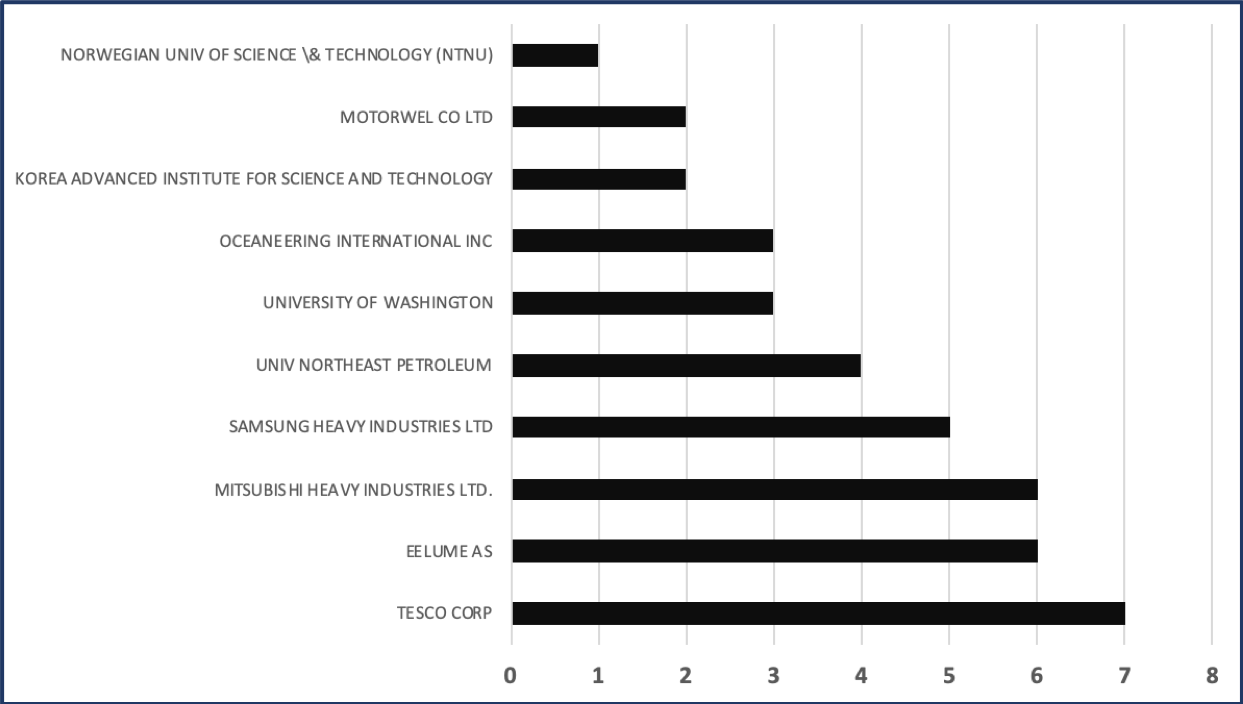
\includegraphics[width=0.9 \textwidth]{images/patenteslist.png} 
  \end{center} 
  \caption{Relação de patentes.} 
  %\legend{Fonte: os autores.} 
  \label{fig:relpat} 
\end{figure}
%\end{sidewaysfigure*}
%----------------------------

% \begin{tikzpicture}
% 	\begin{axis}[title  = Contributions per category
% 							at LaTeX-Community.org,
% 	  xbar,
% 	  y axis line style = { opacity = 0 },
% 	  axis x line       = none,
% 	  tickwidth         = 0pt,
% 	  enlarge y limits  = 0.2,
% 	  enlarge x limits  = 0.02,
% 	  symbolic y coords = {LaTeX, Tools, Distributions, Editors},
% 	  nodes near coords,
% 	]
% 	\addplot coordinates { (57727,LaTeX)         (5672,Tools)
% 						   (2193,Distributions)  (11106,Editors) };
% 	\addplot coordinates { (14320,LaTeX)         (1615,Tools)
% 						   (560,Distributions)   (3075,Editors)  };
% 	\legend{Topics, Posts}
% 	\end{axis}
%   \end{tikzpicture}

A Coréia é o país com maior número de patentes (11 registros), em seguida vem os EUA com 9 registros e a China com 3 patentes.
O relatório apresenta ainda um fato interessante que a grande maioria das patentes encontradas tiveram o seu depótiso no ano de 2017, totalizando em torno de 11 patentes submetidas e registaradas.

A busca também levou em consideração a identificação de artigos científicos relevantes para a pesquisa, os mais relevantes são:  
\begin{itemize}
	\item Research on Underwater Safety Inspection and Operational Robot Motion Control \cite{guangyi2018research};
	\item Augmented reality visualization of scene depth for aiding ROV pilots in underwater manipulation \cite{bruno2018augmented};
	\item Dynamic Modeling and Identification of an Heterogeneously Actuated Underwater Manipulator Arm \cite{leborne2018dynamic};
	\item Design, prototyping and testing of a modular small-sized underwater robotic arm controlled through a Master-Slave approach \cite{barbieri2018design};
	\item Underwater manipulators: A review \cite{sivvcev2018underwater};
	\item A Modular Soft Robotic Wrist for Underwater Manipulation \cite{kurumaya2018modular};
	\item Fully automatic visual servoing control for work-class marine intervention ROVs \cite{sivvcev2018fully};
	\item Collision Detection for Underwater ROV Manipulator Systems \cite{sivvcev2018collision};
	\item Kinematic performances evaluation of a hydraulic underwater manipulator \cite{rizzo2017kinematic};
	\item Impact of Arm Morphology on the Hydrodynamic Behavior of a Two-arm Robotic Marine Vehicle \cite{kazakidi2017impact};
	\item Development of Hand Gesture Recognition Sensor Based on Accelerometer and Gyroscope for Controlling Arm of Underwater Remotely Operated Robot \cite{mardiyanto2017development};
	\item Robust Adaptive PID Control for Positioning of Remotely Operated Vehicle Working in Close Proximity of an Underwater Structure \cite{qiao2016robust};
	\item Development of a Virtual Platform for Telepresence Control of an Underwater Manipulator Mounted on a Submersible Vehicle \cite{zhang2016development};
	\item The Underwater Swimming Manipulator - A Bio-Inspired AUV \cite{sverdrup2016underwater};
	\item Convolutional Neural Network-based Real-time ROV Detection Using Forward-looking Sonar Image \cite{kim2016convolutional};
	\item I-AUV Docking and Panel Intervention at Sea \cite{palomeras2016auv};
	\item 3D-Belief Space Planning for underwater mobile \cite{zereik20153d};
	\item Intervention AUVs: The next challenge \cite{ridao2014intervention};
	\item Rotation Identification in Geometric Algebra: Theory and Application to the Navigation of Underwater Robots in the Field \cite{stanway2015rotation};
	\item I-AUV Docking and Intervention in a Subsea Panel \cite{palomeras2014auv};
	\item Design of Modular Camera Tool for Mini Underwater ROVs \cite{poretti2013design};
	\item Design of a gateway for remotely underwater vehicles \cite{liu2012design};
	\item Stochastic controllers for robust underwater mobile manipulation \cite{bonsignorio2012stochastic};
	\item New Approach for a Reconfigurable Autonomous Underwater Vehicle for Intervention \cite{de2009new};
	\item Manipulability analysis of underwater robotic arms on ROV and application to task-oriented joint configuration \cite{jun2004manipulability};
	\item ArmillEye: Flexible platform for underwater stereo vision \cite{zoppi2007armilleye};
	\item Adaptive PD-controller for positioning of a remotely operated vehicle close to an underwater structure: Theory and experiments \cite{hoang2007adaptive};
	\item A composite rigid body algorithm for modeling and simulation of an underwater vehicle equipped with manipulator arms \cite{hosseini2006composite};
	\item Navigation and control system of a deep-sea unmanned underwater vehicle 'HEMIRE' \cite{lee2007navigation};
	\item Manipulability analysis of underwater robotic arms on ROV and application to task-oriented joint configuration \cite{jun2004manipulability};
	\item A fuzzy approach to redundancy resolution for underwater vehicle-manipulator systems \cite{antonelli2000fuzzy};
	\item Controlling an uninstrumented manipulator by visual servoing \cite{marchand2002controlling};
	\item Control architecture and operator interface for a free-flying robotic vehicle \cite{carignan2001control};
	\item Controlling an uninstrumented ROV manipulator by visual servoing \cite{marchand2001controlling};
	\item Controlling the manipulator of an underwater ROV using a coarse calibrated pan/tilt camera \cite{marchand2001controllingx};
	\item Forestry equipment strikes fear into trees \cite{heney2000features};
	\item Control laws, tasks and procedures with ORCCAD: application to the control of an underwater arm \cite{simon1998control};
	\item Hybrid position/force control of a ROV with a manipulator \cite{lapierre1998hybrid};
	\item A virtual environment for undersea telepresence \cite{schebor1995virtual};
	\item Subsea weld inspection using an advanced robotic manipulator \cite{broome1995subsea};
	\item Experiments in the coordination of underwater manipulator and vehicle control \cite{mclain1995experiments};
	\item Concept evaluation trials of teleoperation system for control of an underwater robotic arm by graphical simulation techniques \cite{boyle1995concept};
	\item Advanced controller for an underwater manipulator \cite{larkum1994advanced};
	\item Planning and control for coordination of underwater manipulators \cite{lane1991planning};
\end{itemize}


%\subsubsection{Benchmarking}
%\label{ssec:benchmani}
%
%\subsubsection{Estudo de comparação das operações de ROV}
%\label{sec:compmani}



\ldots






